\documentclass{article}

\usepackage[utf8]{inputenc}
\usepackage[danish]{babel}
\usepackage{float}
\usepackage{fancyhdr}
\usepackage{amsmath}
\usepackage{color}
\usepackage{listings}
\usepackage{graphicx}
\usepackage{pdfpages}
\usepackage{booktabs}
%\usepackage{enumitem}
\usepackage[a4paper, top = 1in, bottom = 1in, left=1in,right=1in]{geometry}

\title{Exercise 5}
\author{Peter Heilbo Ratgen}
\date{\today}

\begin{document}
\maketitle
Vi laver en summering af variablen \texttt{ames\$Gr.Liv.Area}. 
\begin{lstlisting}
Min. 1st Qu.  Median    Mean 3rd Qu.    Max.
334    1126    1442    1500    1743    5642
\end{lstlisting}
Vi laver også et histogram over denne data.
\begin{figure}[H]
  \centering
  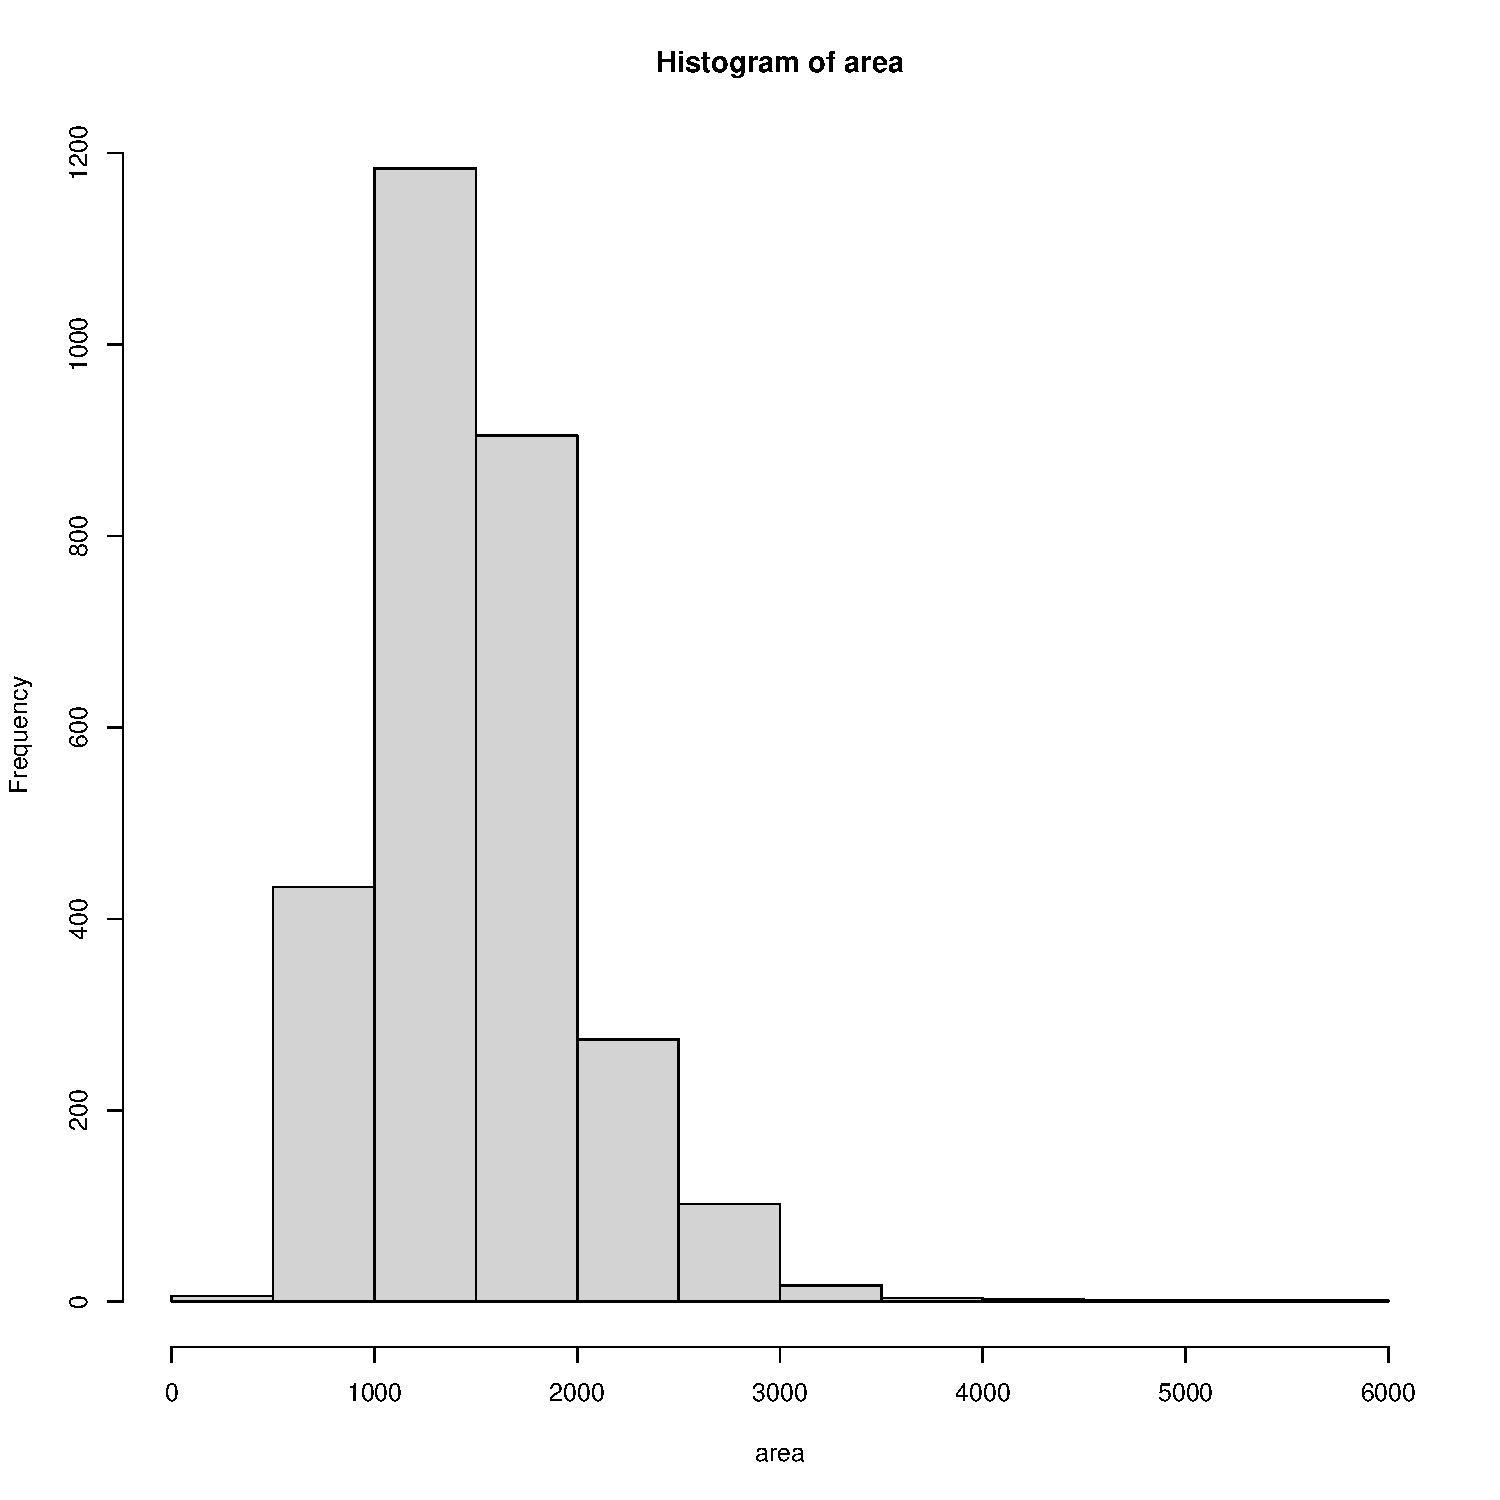
\includegraphics[width=0.65\textwidth]{../area_hist.pdf}
\end{figure}
Her kan vi se at fordelingen er højreskæv, samt at den har den karakteristiske
klokkeform som kendetegner normalfordelingen. 


\end{document}

